%\hypertarget{estilo:capitulo}{}

\chapter{RESULTS AND DISCUSSION} \label{MatMet}

%%%%%%%%%%%%%%%%%%%%%%%%%%%%%%%%%%%%%%%%%%%%%%%%%
The data were processed for the same time window and an exploratory data analysis was performed using the graph below (\ref{fig:graph}). The pluviometric data were collected from the 833A pluviometer, in which the accumulated rain level per day was added. This rain gauge measures the rain level  every 10 minutes. Radar precipitation data was collected in a cell that covers the same region as the pluviometer, thus processing the data for the analyzed temporal window. Tweets were collected within a radius of \si{2000 \meter} and filtered based on a list of words. The words were: 'chuva', 'chove', 'chuvoso', 'chuvosa', according to \cite{de2021effect}, these words are less spatially and temporally volatile than more local and idiosyncratic terms specifically related to the city of São Paulo (e.g. 'garoa' and 'tempestade'). 

\begin{figure}[H]
	\centering
	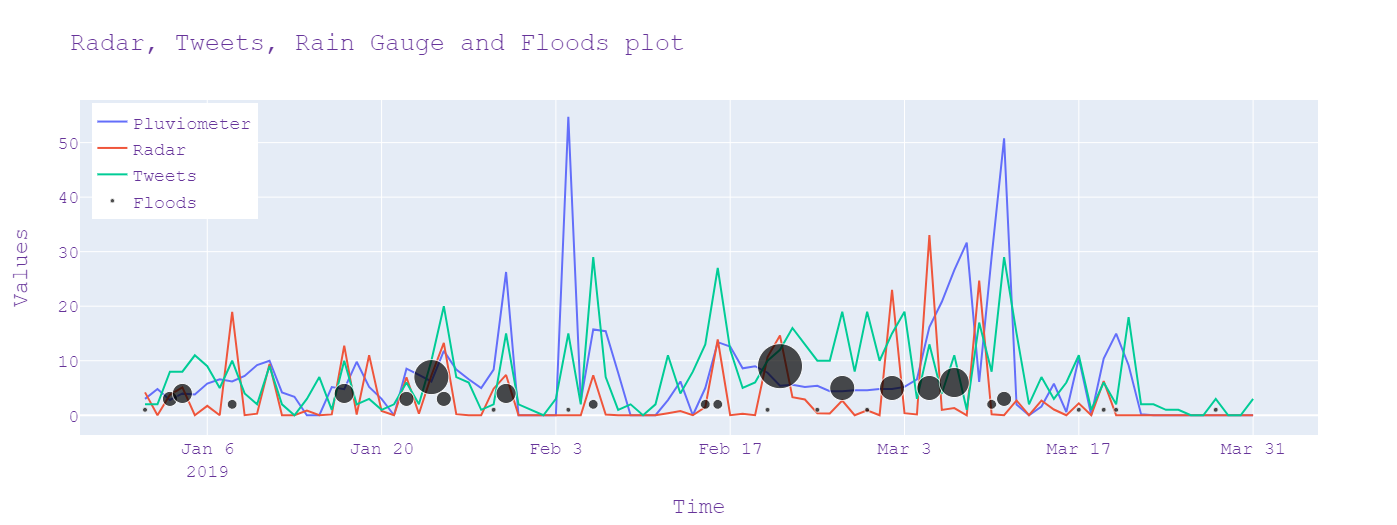
\includegraphics[width=1.2\textwidth]{figs/newplot.png}
	\caption{Plot}
	\label{fig:graph}
\end{figure}

The plotting of data indicates that on every day that flooding occurred there was an incidence of rain indicated by the rain gauge and radar and rain-related tweets. As can be seen in the figure \ref{fig:graph}, the frequency of flooding on a given day determines the size of the black circle, and that the days with the highest incidence of flooding were not peaks of rain detected by meteorological equipment.

To determine the statistical relationships a series of tests were performed. First, it was necessary to determine if the attributes were a normal distribution, so that in this way parametric or non-parametric statistical tests could be applied. For this verification, the Shapiro Wilk test was used (\ref{shapiro}).

\begin{table}[H]\label{shapiro}
	\caption{P-Values results}
	\begin{center}
	\begin{tabular}{ll}
		\hline
		\multicolumn{2}{c}{Shapiro-Wilk test $\alpha=0.05$}                              \\ \hline
		\multicolumn{1}{c|}{Attributes}      & \multicolumn{1}{c}{P-value} \\ \hline
		\multicolumn{1}{l|}{Rain Gauge}      & 7.175038015984347e-13       \\ \hline
		\multicolumn{1}{l|}{Tweet Frequence} & 2.0394061550632614e-07      \\ \hline
		\multicolumn{1}{l|}{Radar}           & 7.194410709808908e-15       \\ \hline
		\multicolumn{1}{l|}{Flood}           & 1.445436313501046e-14       \\ \hline
	\end{tabular}
\end{center}
\end{table}

In the table above \ref{shapiro}, the p-values of all attributes were below the limit of $\alpha$, discarding the null hypothesis that the distribution is normal. Based on the results, to calculate the correlations, Spearman's non-parametric test (\ref{fig:corr}) was used for these data. 

\begin{figure}[H]
	\centering
	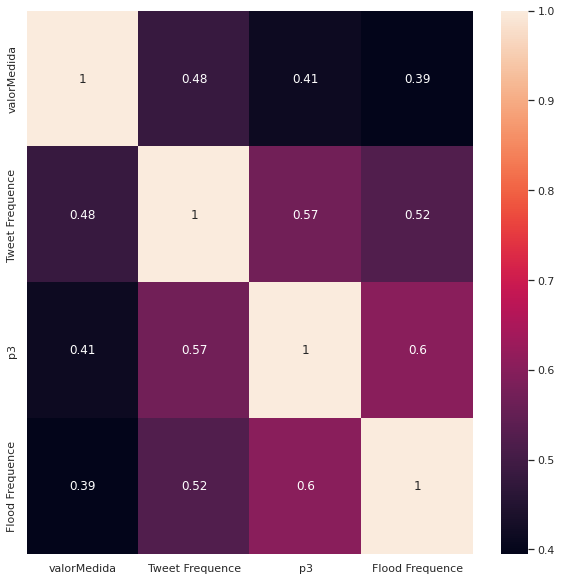
\includegraphics[width=0.47\textwidth]{figs/corr.png}
	\caption{Spearman Correlation}
	\label{fig:corr}
\end{figure}

From the correlations, it is clear that the radar (p3), followed by the tweets, have the highest correlation with the frequency of flooding and also the most significant value. According to \citen{statistics_solutions_2021}, the cited attributes indicates a strong correlation with floods. 

Furthermore, rainfall data indicate low interaction with other attributes. From the results, the most relevant correlations will also exert greater influence on the flooding prediction.
